\documentclass{beamer}

% Add
%  -- generation of authentication key (H)
%  -- field & ring definitions

\usepackage{graphicx}
\usepackage[utf8]{inputenc}

\title{GCM; The illegal attack}
\author{Mathias Hall-Andersen (rot256)}
\institute{Pwnies @ Copenhagen University}
\date{2017}

\begin{document}

\frame{\titlepage}

\begin{frame}
\frametitle{Before we start : Get Sage}

\textbf{Fill your disk} \\
\texttt{docker pull sagemath/sagemath}
\url{https://www.sagemath.org/}

\vspace{3mm}

\textbf{Or, sign up at} \\
\url{https://cocalc.com/}

\end{frame}

\begin{frame}
\frametitle{Mode of operation}
\begin{center}
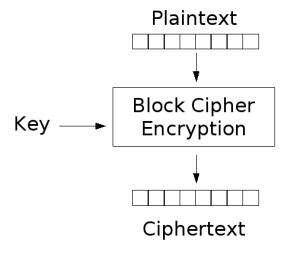
\includegraphics[height=0.5\textheight]{block_cipher.png}
\end{center}
\end{frame}

\begin{frame}
\frametitle{Mode of operation}
\begin{center}
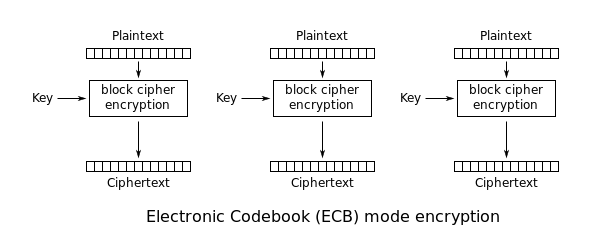
\includegraphics[width=\textwidth]{mode-ecb.png}
\end{center}
\end{frame}

\begin{frame}
\frametitle{Mode of operation}
\begin{center}
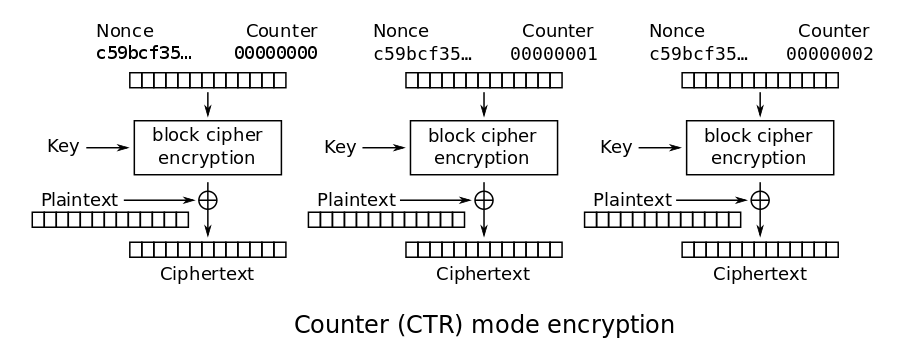
\includegraphics[width=\textwidth]{mode-ctr.png}
\end{center}
\end{frame}

\begin{frame}
\frametitle{Authenticated encryption}
\begin{center}
Encryption $\neq$ Authentication
\end{center}
\end{frame}

\begin{frame}
\frametitle{Galois Counter Mode (motivation)}
\begin{center}
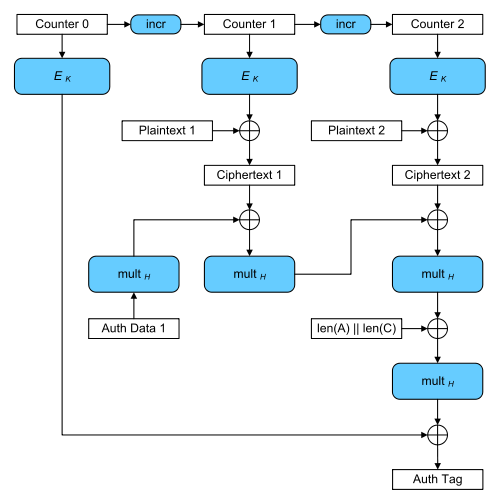
\includegraphics[height=0.8\textheight]{mode-gcm.png}
\end{center}
\end{frame}

\begin{frame}
\frametitle{Galois Counter Mode (motivation)}
\begin{center}
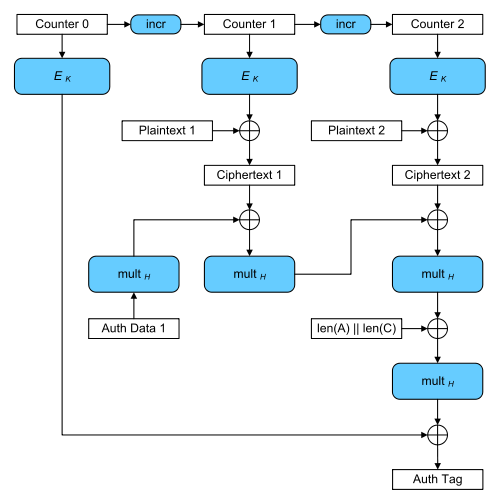
\includegraphics[height=0.8\textheight]{mode-gcm.png}
\end{center}
So what is $mult_{H}(\cdot)$?
\end{frame}

\begin{frame}
\frametitle{Some algebra}
\begin{center}
$mult_{H}(\cdot)$ is multiplication by $H$, \\
but not quite the way you might think...
\end{center}
\end{frame}

\begin{frame}
\frametitle{Rings}
\[
    (E, \cdot, +, 0, 1)
\]
Group + multiplication, e.i.
\[
    z \cdot (x + y)
    =
    z \cdot x
    +
    z \cdot y
\]
\[
    \forall x :
    \exists y :
    x + y = 0
\]
\[
    \forall x :
    x + 0 = x
\]
\[
    \forall x :
    x \cdot 1 = x
\]
Examples:
\[
    \mathbb{Z}
\]
Question: How about $\mathbb{N}_{\geq 0}$?
\end{frame}

\begin{frame}
\frametitle{Fields}
\[
    (E, \cdot, +, 0, 1)
\]
Ring + multiplicative inverses, e.i.
\[
    \forall x \neq 0 : \exists y : x \cdot y = 1
\]
Usually denote $y = x^{-1}$. \\
Examples:
\[
    \mathbb{Q}, \mathbb{R}
\]
Question: How about $\mathbb{Z}$?
\end{frame}

\begin{frame}
\frametitle{Finite fields}
We will primarily be dealing with the field of two elements:
$1, 0$ \\
Where:
\begin{align}
    1 \cdot x &= x \text{ : 1 is the multiplicative identity} \\
    0 + x     &= x \text{ : 0 is the additive identity} \\
    1 + 1     &= 0 \text{ : the field has characteristic 2}
\end{align}
No magic.
Question:
If considered like bits, what common operations does
addition and multiplication in the field correspond to?
What implication does it have for bit-slicing techniques?
\end{frame}

\begin{frame}
\frametitle{Polynomials over fields}
Given a field. We may consider the polynomials over the field. \\
Examples:
\[
    \mathbb{Z}
\]
\end{frame}

\begin{frame}
\frametitle{Fields}
\[
    (E, \cdot, +, 0, 1)
\]
Ring + multiplicative inverses, e.i.
\[
    \forall x \exists y : x \cdot y = 1
\]
Usually denote $y = x^{-1}$. Examples:
\[
    \mathbb{Q}, \mathbb{R}
\]
\end{frame}

\begin{frame}
\frametitle{Finite fields}
We will primarily be dealing with the field of two elements:
$1, 0$ \\
Where:
\begin{align}
    1 \cdot x &= x \text{ : 1 is the multiplicative identity} \\
    0 + x     &= x \text{ : 0 is the additive identity} \\
    1 + 1     &= 0 \text{ : the field has characteristic 2}
\end{align}
No magic.
Question:
If considered like bits, what common operations does
addition and multiplication in the field correspond to?
What implication does it have for bit-slicing techniques?
\end{frame}

\begin{frame}
\frametitle{Polynomials over fields}
Given a field. We may consider the polynomials over the field. \\
E.g. for\ GF(2):
\[
    f(x) = x^{7} + x^{4} + x^{1} + 1
\]
\[
    g(x) = x^{6} + x^{3}
\]
We write this as $\mathbb{F}[x]$
\end{frame}

\begin{frame}
\frametitle{Multiplication of polynomials over GF(2)}
Lets focus on GF(2)[x].

\vspace{3mm}

Addition happens coefficient wise
and multiplication also happens as you would expect:
\[
    f(x) = x^{7} + x^{4} + x^{1} + 1
\]
\[
    g(x) = x^{6} + x^{3}
\]
\[
    f(x) \cdot g(x)
    =
    x^{6} f(x) +
    x^{3} f(x)
    = (x^{13} + x^{10} + x^{7} + x^{6})
    + (x^{10} + x^{7} + x^{4} + x^{3})
\]
\[
    = x^{13} + x^{6} + x^{4} + x^{3}
\]
Question: Recall the definition! Is this a ring?
\end{frame}

\begin{frame}
\frametitle{Multiplication of polynomials over GF(2)}
Lets focus on GF(2)[x].

\vspace{3mm}

\[
    f(x) = x^{7} + x^{4} + x^{1} + 1
\]
\[
    g(x) = x^{6} + x^{3}
\]
Question: We can represent the polynomials as bit strings,
e.g.
$f(x) \sim 10010011$,
$g(x) \sim 01001000$ what does xor of bit strings correspond to in the ring?
What does left shifting of bit strings correspond to?
\end{frame}

\begin{frame}
\frametitle{From GF(2)[x] to GF($2^{128}$)}

Take my word for it:
We can transform the ring of polynomials into a field by reducing
modulo a particular class of polynomials in the ring, so called `primitive' polynomials.

\vspace{3mm}

For instance $GF(2)[x] \to GF(2^{4})$, by reducing modulo $x^{2} + 1$:
Since $ f = (x^{5} + x^{3} + x^{2} + x + 1) (x^{2} + 1)$, $f \cong 0 \mod x^{2} + 1$
$ g = (x^{4} + x^{2} + x + 1) \cdot (x^{2} + 1) + (x + 1)$, $g \cong x + 1 \mod x^{2} + 1$

\end{frame}

\begin{frame}
\frametitle{From GF(2)[x] to GF($2^{128}$)}
Reduction in GF(2)[x] / p(x). Easy!
\end{frame}

\begin{frame}
\frametitle{Additional resources}
So $mult_{H}(\cdot) : GF(2^{128}) \to GF(2^{128})$ \\
\vspace{3mm}
\textbf{Courses}
\begin{itemize}
    \item Algebra 1 @ Department of Mathematical Sciences (UCPH)
    \item Algebra 2 @ Department of Mathematical Sciences (UCPH)
    \item Computational Discrete Math @ DTU
\end{itemize}
\textbf{Books}
\begin{itemize}
    \item Algebra (2nd Edition) : Micheal Artin
    \item Abstract Algebra : Dummit \& Foote
\end{itemize}
Break?
\end{frame}

\begin{frame}[fragile]
\frametitle{Galois Counter Mode (MAC calculation)}
Authentication key $H \in GF(2^{128})$. \\
Output blocks: $ct_{1}, ct_{2}, \ldots, ct_{n}$ (last padded with zero) \\
Make a block: $len(A) || len(C)$ (length in bits) \\

\vspace{3mm}

For every block add, then multiply with the authentication key.
Basically:
\texttt{foldl (\textbackslash a x -> (a + x) * H) 0 cs}

\vspace{3mm}

Finally add a random (encrypted nonce \verb!||! 0): $E_{k}$
\end{frame}

\begin{frame}
\begin{center}
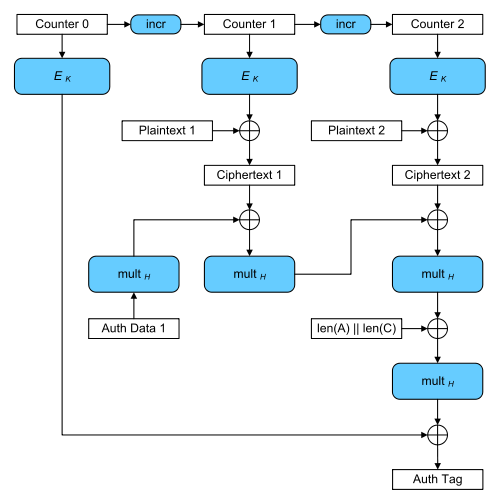
\includegraphics[height=0.9\textheight]{mode-gcm.png}
\end{center}
\end{frame}

\begin{frame}
\frametitle{Galois Counter Mode (MAC calculation)}
Alternatively we can consider it as evaluation the polynomial:
\[
    w(y) = c_{1} y^{n} + \ldots + c_{n} y^{2} + c_{n+1} y^{1} + E_{k} \in GF(2^{128})[y]
\]
At $H$, e.i. $T = w(H)$.
This will be useful.
\end{frame}

\begin{frame}
\frametitle{Galois Counter Mode (MAC calculation)}
Consider the case where, the MAC is computed on two different messages $c$, $c'$,
but $E_{k} = E'_{k}$.
We know:
\[
    T = w(H) = c_{1} H^{n} + \ldots + c_{n} H^{2} + c_{n+1} H^{1} + E_{k}
\]
\[
    T' = w'(H) = c'_{1} H^{m} + \ldots + c'_{m} H^{2} + c'_{m+1} H^{1} + E_{k}
\]
Move terms over:
\[
    0 = c_{1} H^{n} + \ldots + c_{n} H^{2} + c_{n+1} H^{1} + E_{k} + w(H)
\]
\[
    0 = c'_{1} H^{m} + \ldots + c'_{m} H^{2} + c'_{m+1} H^{1} + E_{k} + w'(H)
\]
\end{frame}

\begin{frame}
\frametitle{Galois Counter Mode (MAC calculation)}
\[
    0 = c_{1} H^{n} + \ldots + c_{n} H^{2} + c_{n+1} H^{1} + E_{k} + w(H)
\]
\[
    0 = c'_{1} H^{m} + \ldots + c'_{m} H^{2} + c'_{m+1} H^{1} + E_{k} + w'(H)
\]
Subtract:
\begin{align}
    0 &=
    (c_{1} H^{n} + \ldots + c_{n} H^{2} + c_{n+1} H^{1} + E_{k} + w(H)) - \\
    & \ \ \ \ (c'_{1} H^{m} + \ldots + c'_{m} H^{2} + c'_{m+1} H^{1} + E_{k} + w'(H)) \\
    &=(c_{1} H^{n} + \ldots + c_{n} H^{2} + c_{n+1} H^{1} + w(H)) + \\
    & \ \ \ \ (c'_{1} H^{m} + \ldots + c'_{m} H^{2} + c'_{m+1} H^{1} + w'(H))
\end{align}
So $H$ is a root of $(w(y) - T) - (w'(y) - T')$. Easy?
\end{frame}

\begin{frame}
\frametitle{SageMath}
`SageMath is a free open-source mathematics software system licensed under the GPL.
 It builds on top of many existing open-source packages:
 NumPy, SciPy, matplotlib, Sympy, Maxima, GAP, FLINT, R and many more'
 - \url{https://www.sagemath.org/}
\end{frame}

\begin{frame}[fragile]
\frametitle{Work session}

Go to \url{http://rot256.io:8080} for the challenge.

\vspace{3mm}

The algebraic structures we will be needing in Sage:

\begin{verbatim}
F.<x> = GF(2^128, 'x', x^128 + x^7 + x^2 + x + 1)
G.<y> = PolynomialRing(F)
\end{verbatim}

There is a \verb!doit.sage! template at \url{https://rot256.io/doit.sage}. \\
Containing useful helpers if you wish to use these in the attack.

\end{frame}

\end{document}
